
\chapter{Belgische bedrijven en IPv6}
\label{ch:h6}

\section{IPv6 Adoptie}

Op onderstaande afbeelding van Google is er te zien dat België momenteel een IPv6 adoptie heeft van 52.22\%. Dit wil zeggen dat 52.22\% van de gebruikers IPv6 connectie gebruikt om over Google te surfen. Dus meer dan de helft van het verkeer gaat over IPv6. Volgens de statistieken van Google is België het hoogste land met zoveel IPv6 connectiviteit. Hoe groener het land, hoe groter de adoptie. Terwijl het wereldwijde aantal maar 20.74\% bevat. Dan heeft België meer dan het dubbele aantal dan het wereldwijde gebruik. Dit maakt België het land met het hoogste aantal IPv6 gebruikers van de wereld.

\begin{figure}
\centering
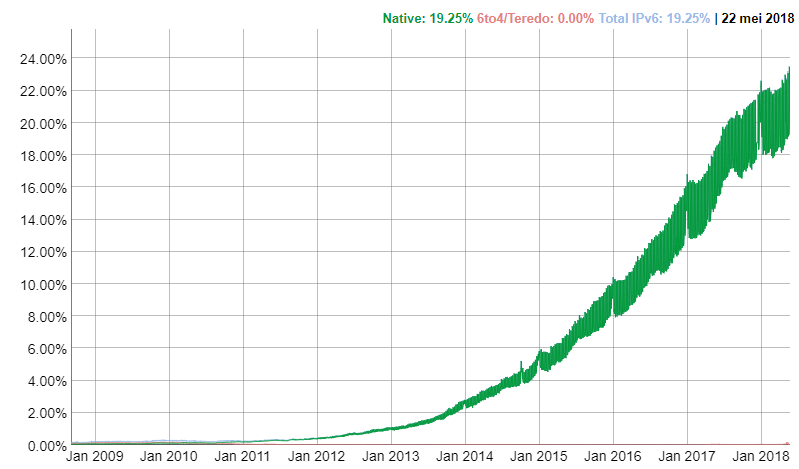
\includegraphics[width=\textwidth,height=\textheight,keepaspectratio]{googleIPv6.png}
\caption{IPv6 status IPv6 in België \autocite{GoogleIPv6Belgie}}
\end{figure}

Nog belangrijk om na te gaan zijn de webbrowsers die IPv6 bereikbaar maken. Dit is een zeer belangrijk element en zeker voor de Belgische bedrijven. Omdat meer en meer gebruik wordt gemaakt van IPv6 en er vaak nog alleen IPv6 gebruikt wordt, is het belangrijk dat bedrijven zich hieraan gaan aanpassen. Als een website van een webshop enkel via IPv4 bereikbaar is dan kunnen de IPv6 klanten geen online shoppingen doen bij deze winkel. Hiervoor is het belangrijk dat bedrijven er zich van bewust zijn dat de webbrowsers zowel IPv4 als IPv6 toegankelijk moeten maken. In onderstaande grafiek is er te zien wat de status is van IPv6 toegankelijke webbrowsers en hoe de evolutie hiervan in de toekomst geschat kan worden. Om de evolutie hiervan te berekenen is er gebruik gemaakt van een logistische s-curve en een voorspelling op de komende 4 jaar of 1460 dagen. Op 26 mei waren er 52.27\% van de sites IPv6 toegankelijk. Volgens de berekeningen zal de 90\% behaald worden op 9 mei 2019, of minder dan 1 jaar zou er 90\% van de Belgische webbrowsers IPv6 actief moeten zijn.

\begin{figure}
\centering
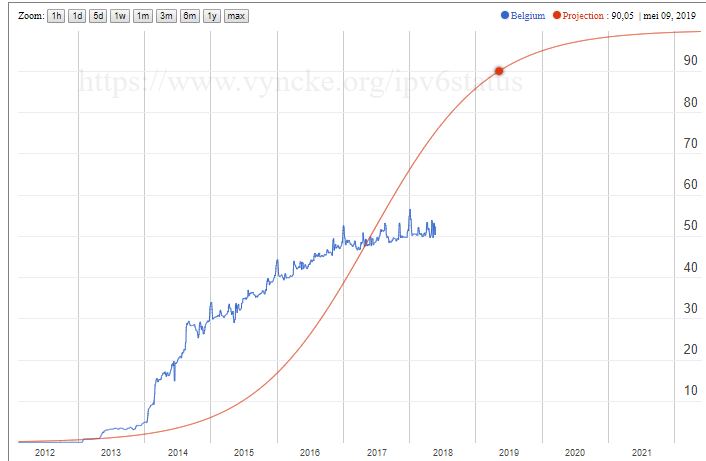
\includegraphics[width=\textwidth,height=\textheight,keepaspectratio]{IPv6vervolg.png}
\caption{IPv6 vervolg op 4 jaar \autocite{Vyncke2018}}
\end{figure}

Het is alvast zeker dat België het beste presteert op het aantal gebruikers over IPv6. Nu rest er enkel nog de vraag waarom België meer gebruikers heeft dan eender welk land. Voor deze vraag heeft Eric Vyncke, mede-eigenaar van de Belgische IPv6 Council, een mogelijk antwoord. Het biedt enkele mogelijkheden die een rol kunnen spelen waarom België zo’n hoog percentage behaald. De eerste mogelijkheid is er omdat België een vrij klein land is en dicht bevolkt. Omdat het land vrij klein is, is de afstand dus ook klein. Daarom wordt er ook vaak gebruik gemaakt van kabel of xDSL aansluitingen. Ook omdat veel van de Belgische ISP’s een tekort hadden aan IPv4 adressen, was er snel een oplossing door gebruik te maken van IPv6. Ook is er een soort van geheim tussen de verschillende ISP’s, cyberpolitie, regelgevers en de minister van economische zaken om het delen van 1 IPv4 adres maximum te beperken tot 16 abonnees. Dit had een grote invloed op het gebruik van NAT/CGN. Als de cultuur van België nader wordt bekeken dan is het een mix van zowel een Duitse als Latijnse cultuur. Dit wil ook zeggen dat er vaak gekeken wordt op een langere termijn en dat er niet veel wordt aangetrokken rond de processen. Ook hebben de drie grote ISP’s van België samengezeten om het gebruik van IPv6 te verduidelijken. Hierbij hebben ze vooral ervaring en een routekaart  met elkaar gedeeld om de evolutie te vergemakkelijken. Dit zijn enkele redenen volgens Eric Vyncke, waarbij hijzelf zegt dat er geen duidelijke reden hiervoor is en dit enkel maar veronderstellingen zijn.

\section{Enquête aan Belgische bedrijven}

Voor een breder beeld te krijgen over hoe het er in sommige bedrijven aan toe zijn, is er een enquête opgestuurd naar verschillende experten. De enquête en opgestelde vragen kan u terugvinden in de bijlagen om de corpus van de scriptie te bewaren. Deze vragen zijn vooral gericht op hoe het bedrijf er tegenover staat, IPv6. Het intern netwerk draaiende op IPv4, IPv6 of beiden. Hoe het zit met de kennis over IPv6, advies geven hiervan, begrippen herkennen en meer. Om de resultaten samen te vatten is er te merken dat er nog geen geval is van een IPv6 only intern netwerk. Zowel IPv4 als een IPv4/IPv6 structuur is al te vinden in een intern netwerk van bedrijven. Als er dan eerder de vraag werd gesteld of er toekomst plannen waren voor een mogelijke implementatie dan kwam er ook de respons dat ze er nog niet mee bezig waren en nog niet aan dachten om dit te implementeren in hun netwerk. Met de vraag of ze zouden kiezen voor een IPv4/IPv6 of een IPv6 structuur, dan kwam er een duidelijk antwoord dat ze allemaal voor gemengd kozen. Dit omdat men de overgang in een langzame beweging zouden volbrengen en omdat IPv4 nog steeds populair blijft. Alsook omdat niet al het apparatuur IPv6 compatibel is in vele gevallen. Er werd ook een bedrijf ondervraagd dat niet hoofdzakelijk met ICT diensten bezig is maar wel hun eigen afdeling heeft. Zij zouden voor deze overschakeling grotendeels gebruik maken van hun interne werkkracht maar zouden toch nog extra externe expertise raadplegen terwijl bij een IT consultancy bedrijf genoeg interne werkkracht heeft met de kennis van IPv6. Als er werd nagegaan over de kennis van IPv6, door het ondervragen van een begrip namelijk SLAAC, dan had niemand daar een probleem mee deze ook te beantwoorden. Wat wil leiden tot een beginkennis van IPv6. De voornaamste redenen om de overschakeling nog niet te beginnen is vooral door de complexiteit van de overgang en kennis van de engineers. Maar ook omdat sommige infrastructuren er nog niet klaar voor of nog niet compatibel hiermee zijn. Wat ook een reden was dat klanten geen nieuwe investeringen willen doen in de ICT infrastructuur en zeker nog niet met de start van GDPR (General Data Protection Regulation). Als ze zichzelf een score op 5 moeten geven dan scoort deze maximaal 2.5/5 voor kennis in IPv6. Dit toont nogmaals aan dat er te weinig opleidingen en opvolging is van het nieuwe internet protocol. Hierin zal in de toekomst meer geïnvesteerd moeten worden als men hiermee meer te maken zal hebben. Ook is er gevraagd geweest naar de toegankelijkheid van hun webbrowsers. We hebben zowel het antwoord ja als nee gekregen. Dit toont erop aan dat men toch rekening aan het houden is met de toegankelijkheid van hun sites. Ook bij degenen waarbij ze nog niet IPv6 actief zijn, blijft het antwoord dat het momenteel nog niet zo is, wat wil duiden op toekomstige plannen. De laatste vraag die besproken zal worden gaat over hoe ze in aanraking gekomen zijn met IPv6. We zien hierbij vooral dat er toch al trainingen en seminaries worden gevolgd. Alsook het behalen van certificaten en in contact komen met partners en datacenters. Ook bij de twee grootste Belgische IPS’s, Telenet en Proximus, is het mogelijk om als klant gebruikt te maken van IPv6. Als men thuis een IPv6 verbinding wilt hebben dan bieden ze beiden ook een zeer goede ondersteuning hiervoor aan.

Een besluit die we hieruit kunnen trekken is dat er toch al bedrijven actief met IPv6 aan het werken zijn maar eerder gedeeld met IPv4. Dit maakt het ook beter om al een ruimere kennis op te doen. Ook is eruit af te leiden dat de kennis totaal nog niet op een hoog punt staat, maar dat er gezegd kan worden dat er trainingen gevolgd worden. 
